\documentclass[UTF8]{ctexart}
\usepackage[a4paper,left=3cm,right=3cm,top=2cm]{geometry}
\usepackage{amsmath}
\usepackage{enumitem}
\usepackage{float}
\usepackage{threeparttable}
\usepackage{caption}
\usepackage{multirow}
\usepackage{graphicx}
\usepackage{color}


\definecolor{dkgreen}{rgb}{0,0.6,0}
\definecolor{gray}{rgb}{0.5,0.5,0.5}
\definecolor{mauve}{rgb}{0.58,0,0.82}

\setlength\lineskiplimit{5.25bp}
\setlength\lineskip{5.25bp}

\title{凯特摆实验报告}
\author{崔士强 PB22151743}
\date{\today}

\bibliographystyle{plain}

\begin{document}
\maketitle
\begin{abstract}
  本实验利用凯特摆共轭点的特性测量重力加速度. 实验中对凯特摆等效摆长$l$,
  两个转轴对应的周期$T_1$, $T_2$,以及转轴到重心的距离进行测量,最终测得重力加速度$g=\left(9.7585 \pm 0.02\right)\mathrm{m/s^2}$.
  本实验的误差主要来源于$T_1$与$T_2$并不严格相等,以及在测量过程中存在的误差,后者为主要因素.
\end{abstract}

关键词:凯特摆,重力加速度.

\section{引言}
对于一复摆,设其质量为$m$,转轴为$O$,绕$O$的转动惯量为$I$,$O$到重心$G$的距离为$h$,则有:
\[T = 2\pi \sqrt{\frac{I}{mgh}}\]

设复摆绕平行于$O$轴并且通过重心$G$的转动惯量为$I_G$,根据平行轴定理则有:
\[T = 2\pi \sqrt{\frac{I_G+mh^2}{mgh}}\]

可设等效摆长
\[l = \frac{I_G+mh^2}{mh}\]

若测出周期以及等效摆长则可测出重力加速度. 由复摆的共轭特性可以知道,
在复摆重心两侧, 并且和重心处于同一条直线上的两个点$O$, $O'$,
分别测量以$O$, $O'$为悬点的摆动周期$T_1$, $T_2$, 当$T_1$, $T_2$相等时, $OO'$就是等效摆长.

\begin{figure}[H]
  \centering
  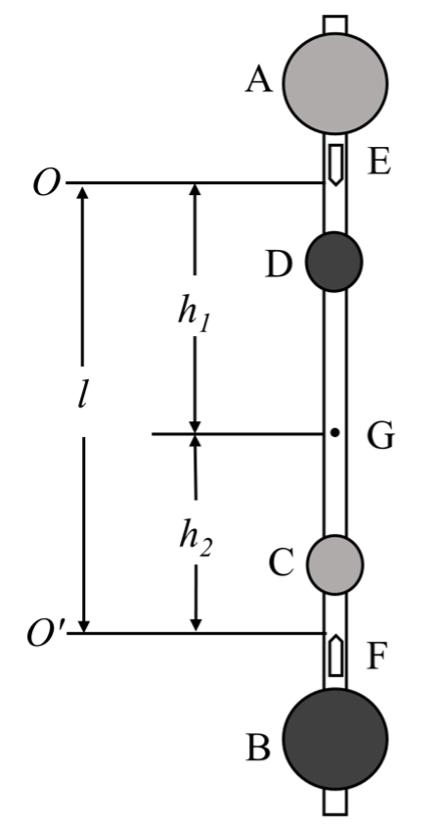
\includegraphics[scale=0.7]{p1.png}
  \caption{凯特摆示意图}
\end{figure}

在如图1所示的凯特摆中通过调节A, B, C, D的位置可以使以$O$, $O'$为悬点的摆动周期相等,此时有:
\[T_1 = 2\pi \sqrt{\frac{I_G+mh_1^2}{mgh_1}}\]
\[T_1 = 2\pi \sqrt{\frac{I_G+mh_2^2}{mgh_2}}\]

消去$I_G$可得:
\[\frac{4 \pi^2}{g} = \frac{T_1^2+T_2^2}{2l}+\frac{T_1^2-T_2^2}{2\left(h_1-h_2\right)}\]

实验中由于凯特摆的不对称设计,第二项很小,同时减小了其带来的误差.
\section{实验}
\subsection{实验仪器}
本实验所用仪器包括凯特摆,光电探头,多用数字测试仪,钢卷尺.

其中钢卷尺的最大允差$\Delta_{app}=0.2\mathrm{cm}$, 估计误差$\Delta_{est}=0.05\mathrm{cm}$. 
多用数字测试仪的最大允差$\Delta_{app}=0.0001\mathrm{s}$.
\subsection{数据}
实验中测量了$T_1$, $T_2$, $h_1$, $l$的值,数据如下表所示:
\begin{table}[H]
  \centering
  \begin{tabular}{cccc}
    \hline\hline
    $10T_1(\mathrm{s})$ & $10T_2(\mathrm{s})$ & $h_1(\mathrm{cm})$ & $l(\mathrm{cm})$ \\
    \hline
    17.3992 & 17.3938 & 30.30 & 74.70 \\
    17.3998 & 17.3956 & 30.28 & 74.69 \\
    17.3951 & 17.3948 & 30.33 & 74.70 \\
    17.4026 & 17.3951 & & \\
    17.4017 & 17.3942 & & \\
    \hline\hline
  \end{tabular}
  \caption{实验数据}
\end{table}
\section{实验结果讨论}
\subsection{数据分析}
$T_1$的平均值
\[\overline{T_1} = \frac{1}{10n}\sum_{n=1}^{5} 10 T_{1_n} = 1.73997\mathrm{s}\]

$T_1$的标准差
\[\sigma_{T_1} = \sqrt{\frac{1}{n-1}\sum_{n=1}^{5}\left(T_{1_n}-\overline{T_1}\right)^2} = 2.60108\times 10^{-4}\mathrm{s}\]

$T_2$的平均值
\[\overline{T_2} = \frac{1}{10n}\sum_{n=1}^{5} 10 T_{2_n} = 1.73947\mathrm{s}\]

$T_2$的标准差
\[\sigma_{T_2} = \sqrt{\frac{1}{n-1}\sum_{n=1}^{5}\left(T_{2_n}-\overline{T_2}\right)^2} = 6.38749\times 10^{-5}\mathrm{s}\]

$T$的B类不确定度
\[\Delta_{B,T}=10^{-5}\mathrm{s}\]

$T_1$的展伸不确定度
\[U_{T_1, P}=\sqrt{\left(t_P\frac{\sigma_{T_1}}{\sqrt{n}}\right)^2+\left(k_P\frac{\Delta_{B,T}}{C}\right)^2}=3.23446\times 10^{-4}\mathrm{s}, P=0.95\]

$T_2$的展伸不确定度
\[U_{T_2, P}=\sqrt{\left(t_P\frac{\sigma_{T_2}}{\sqrt{n}}\right)^2+\left(k_P\frac{\Delta_{B,T}}{C}\right)^2}=7.96810\times 10^{-5}\mathrm{s}, P=0.95\]

$h_1$的平均值
\[\overline{h_1} = \frac{1}{n}\sum_{n=1}^{3} h_{1_n} = 30.30\mathrm{cm}\]

$h_1$的标准差
\[\sigma_{h_1} = \sqrt{\frac{1}{n-1}\sum_{n=1}^{3}\left(h_{1_n}-\overline{h_1}\right)^2} = 2.055\times 10^{-2}\mathrm{cm}\]

$h_1$的B类不确定度
\[\Delta_{B,h_1} = \sqrt{\left(\frac{\Delta_{app}}{10}\right)^2 + \left(\frac{\Delta_{est}}{10}\right)^2}=0.206155\mathrm{cm}\]

$h_1$的展伸不确定度
\[U_{h_1, P}=\sqrt{\left(t_P\frac{\sigma_{h_1}}{\sqrt{n}}\right)^2+\left(k_P\frac{\Delta_{B,h_1}}{C}\right)^2}=0.138668\mathrm{cm}, P=0.95\]

$l$的平均值
\[\overline{l} = \frac{1}{n}\sum_{n=1}^{3} h_{l} = 74.70\mathrm{cm}\]

$l$的标准差
\[\sigma_{l} = \sqrt{\frac{1}{n-1}\sum_{n=1}^{3}\left(l_n-\overline{l}\right)^2} = 4.714\times 10^{-2}\mathrm{cm}\]

$l$的B类不确定度
\[\Delta_{B,l} = \sqrt{\left(\frac{\Delta_{app}}{10}\right)^2 + \left(\frac{\Delta_{est}}{10}\right)^2}=0.206155\mathrm{cm}\]

$l$的展伸不确定度
\[U_{l, P}=\sqrt{\left(t_P\frac{\sigma_{l}}{\sqrt{n}}\right)^2+\left(k_P\frac{\Delta_{B,l}}{C}\right)^2}=0.154484\mathrm{cm}, P=0.95\]

由以上数据可得
\[g = 9.7585\mathrm{m/s^2}\]

g的不确定度
\[U_{g,P}=\sqrt{\left(\frac{\partial g}{\partial l}U_{l,P}\right)^2+\left(\frac{\partial g}{\partial T_1}U_{T_1,P}\right)^2+\left(\frac{\partial g}{\partial T_2}U_{T_2,P}\right)^2}=0.020272\mathrm{m/s^2}\]

最终测量结果
\[g=\left(9.7585 \pm 0.02\right)\mathrm{m/s^2}\]

相对合肥地区重力加速度参考值$g=9.7947\mathrm{m/s^2}$误差为$0.37\%$

\subsection{误差分析}
本实验的误差来源如下
\begin{enumerate}
  \item $T_1$与$T_2$并不严格相等. 这个误差可以通过增大$h_1$与$h_2$的差值来减小.
  \item 在各个物理量的测量过程中存在误差,这里主要是钢卷尺测量$l$和$h_1$的误差.
  \item $h_1$的确定需要找到凯特摆的重心,这个过程中存在误差.
\end{enumerate}

\section{总结}
\subsection{实验总结}
本实验利用凯特摆共轭点的特性测量重力加速度. 实验中对凯特摆等效摆长$l$,
两个转轴对应的周期$T_1$, $T_2$进行测量,最终测得重力加速度$g=\left(9.7585 \pm 0.02\right)\mathrm{m/s^2}$.
本实验的误差主要来源于$T_1$与$T_2$并不严格相等,以及在测量过程中存在的误差,推测后者为主要因素.
\subsection{思考题}
\begin{enumerate}
  \item 实验设计上的特点为通过改变一些物理量来降低误差;另外利用复摆的共轭特性避免了转动惯量的测量;降低了摆长的测量精度;利用凯特摆的不对称设计实现.
  \item 影响精度的主要因素为长度的测量. 与参考值对比,测量值偏小,可能是由于等效摆长的测量值偏小导致.
\end{enumerate}

\begin{thebibliography}{100}
  \bibitem{ref1} 谢行恕,康士秀,霍剑青. 大学物理实验. 北京: 高等教育出版社, 2005.11: 8-11.
  \bibitem{ref2} 王红理,俞晓红,肖国宏. 大学物理实验. 西安:西安交通大学出版社,2014.8,94-97.
  \bibitem{ref3} 沙振舜,周进,周非. 当代物理实验手册. 南京:南京大学出版社,2012.1,36-37.
  \bibitem{ref4} 袁长坤,张静华,袁文峰. 物理量测量. 北京: 科学出版社,2014.12,51-54.
  \bibitem{ref5} 潘之胜,冯璧华,于瑶. 大学物理实验(第二册). 南京:南京大学出版社,2004.01, 23-26.
  \bibitem{ref6} 杨述武,孙迎春,沈国土,赵立竹. 普通物理实验(1). 北京:高等教育出版社,2016.3,81-83.
  \bibitem{ref7} 吕斯骅 段家忯. 新编基础物理实验. 北京:北京高等教育出版社,2006.1,122-127.

\end{thebibliography}

\bibliographystyle{math}

\end{document}
\iffalse
\begin{figure}[h]
    \centering
    \includegraphics[scale=0.5]{name.png}
    \caption{name}
\end{figure}
\fi
